\chapter{Tecnologías para el desarrollo. Hardware y Software.}
\label{chap:tecnologias}

\noindent
\drop{E}n este capítulo son detallados los componentes \emph{hardware} que han sido utilizados para realizar la plataforma de juego, así como las funciones y datos técnicos de los componentes. Son detallados los pasos a seguir para la configuración, instalación y conexionado de cada uno de los dispositivos. Se exponen el conjunto de herramientas \emph{software} empleadas para desarrollar los programas que manejan la plataforma de juego, cuya finalidad es conseguir un entorno gráfico, tangible e intuitivo para el usuario final.


\section{Hardware.}
\label{sec:hardware}
Se conoce como \emph{hardware}, al conjunto de elementos físicos que trabajan conjuntamente como unidad, y que componen un sistema informático.

El cometido principal de los dispositivos \emph{hardware}, es automatizar la plataforma de juego aplicando la electrónica, para controlar distintas funciones y operaciones, trabajando todos los elementos en unidad.
Los dispositivos empleados en la plataforma de juego son los siguientes:
\begin{itemize}
\item Ordenador de placa reducida \emph{Raspberry Pi}. Encargado de administrar y procesar ordenes y eventos dentro del sistema, así como controlar el funcionamiento del resto de los dispositivos \emph{hardware}.
\item Pantallas táctiles. Parte fundamental de la interfaz gráfica e interfaz tangible, para poder visualizar el desarrollo del juego.
\item Sensores. Para mejorar la experiencia de juego, son incorporados un sensor de color, y una unidad de medición inercial.
\end{itemize}

\subsection{Raspberry Pi 3.}
\label{subsubs:rasp}
\emph{Raspberry Pi} es un dispositivo \emph{hardware}, de placa única y bajo coste, diseñado para promover la programación en edades tempranas, y empleado para diversas aplicaciones en proyectos de electrónica~\cite{Upton}.\

El proyecto \emph{Raspberry Pi}, fue creado en 2006 en Reino Unido, por el grupo \emph{Computer Lab} de la Universidad de Cambridge, con el objetivo de estimular la enseñanza de \emph{Ciencias de la Computación} en las escuelas ~\cite{Upton}.

En la actualizad este dispositivo se ha popularizado en todo el mundo, contando con una gran comunidad de usuarios, los cuales aportan tutoriales y documentación, que son de gran ayuda a la hora de emprender un proyecto con este dispositivo. 

El modelo B de \emph{Raspberry Pi 3}, utilizado para este proyecto, aparece en marzo de 2016. Incorpora un procesador diseñado específicamente para ese dispositivo, el \emph{BCM2837 (quad-core Cortex-A53) a 1.2GHz}, que supone un cambio importante, al utilizar una arquitectura de 64bits, a diferencia de los modelos anteriores que aplican una arquitectura de 32bits. Este procesador, además, dispone de un módulo de implementación para las comunicaciones inalámbricas, el \emph{BCM43438}. Incluye un \emph{BCM WiFi 802.11n, Bluetooth LE y Bluetooth 4.1 Classic}.
Este modelo dispone de un cabezal de 40 pines \emph{GPIO}\footnote{General-Purpose Input/Output}, dentro de los cuales se encuentran las conexiones para los buses de datos serie \emph{SPI, I2C y UART}. La Figura~\ref{fig:pinsraspberry} muestra la correspondencia con cada uno de los pines.
La alimentación del dispositivo se realiza por medio de una fuente de alimentación externa (5VDC), vía Micro USB o \emph{GPIO}.

\begin{figure}[!h]
\begin{center}
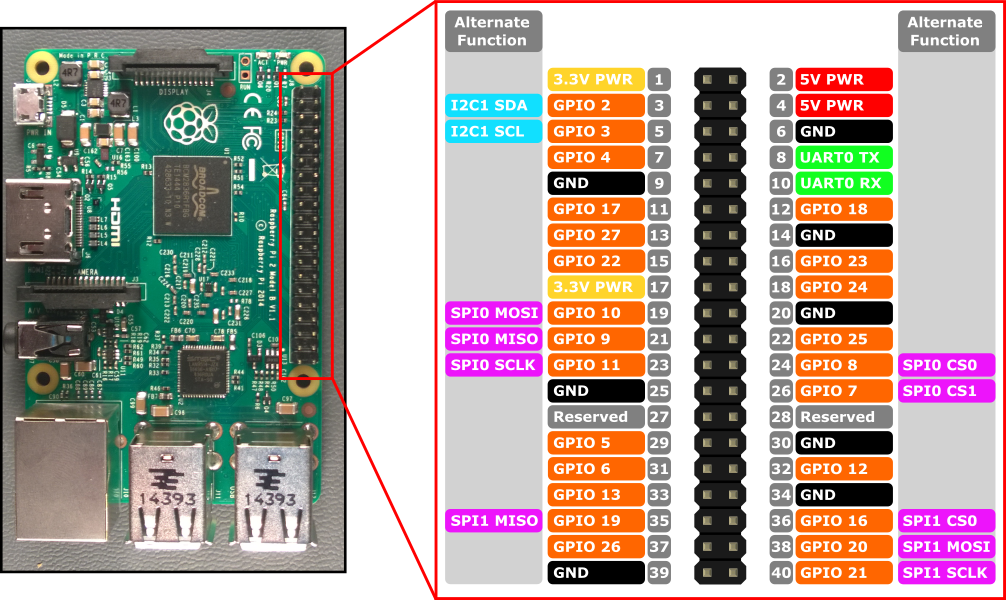
\includegraphics[width=0.8\textwidth]{pinsraspberry.png}
\caption{Pinout Raspberry Pi 3B. Fuente: ~\cite{Upton}}
\label{fig:pinsraspberry}
\end{center}
\end{figure}

\subsubsection{Datos técnicos de \emph{Raspberry Pi 3B}}

A continuación, se muestran las características de la placa \emph{Raspberry Pi 3B}:
\begin{itemize}
\item Procesador BCM2837 quad-core Cortex-A53 a 1.2GHz.
\item VideoCore IV multimedia 400MHz . 
\item Memoria RAM de 1GB.
\item BCM43438 WiFi 802.11n, Bluetooth LE y Bluetooth 4.1 Classic.
\item Controlador SMSC LAN9514 USB/Ethernet
\item Cabecera 40 pines GPIO.
\item Ranura MicroSD para memoria flash.
\item Puerto DSI\footnote{Display Serial Interface.} dedicado a pantalla táctil de Raspberry Pi.
\item Puerto CSI\footnote{Camera Serial Interface.} para cámara de Raspberry Pi.
\item Puerto de salida HDMI.
\item Entrada de alimentación Micro USB.
\item 4 puertos USB 2.0.
\item Puerto Ethernet 10/100, RJ-45.
\item Salida de audio compuesto, conexión tipo Jack de 3.5mm.
\end{itemize}.

Las características han sido obtenidas de \textbf{Raspberry Pi User Guide ~\cite{Upton}}

\begin{figure}[!h]
\begin{center}
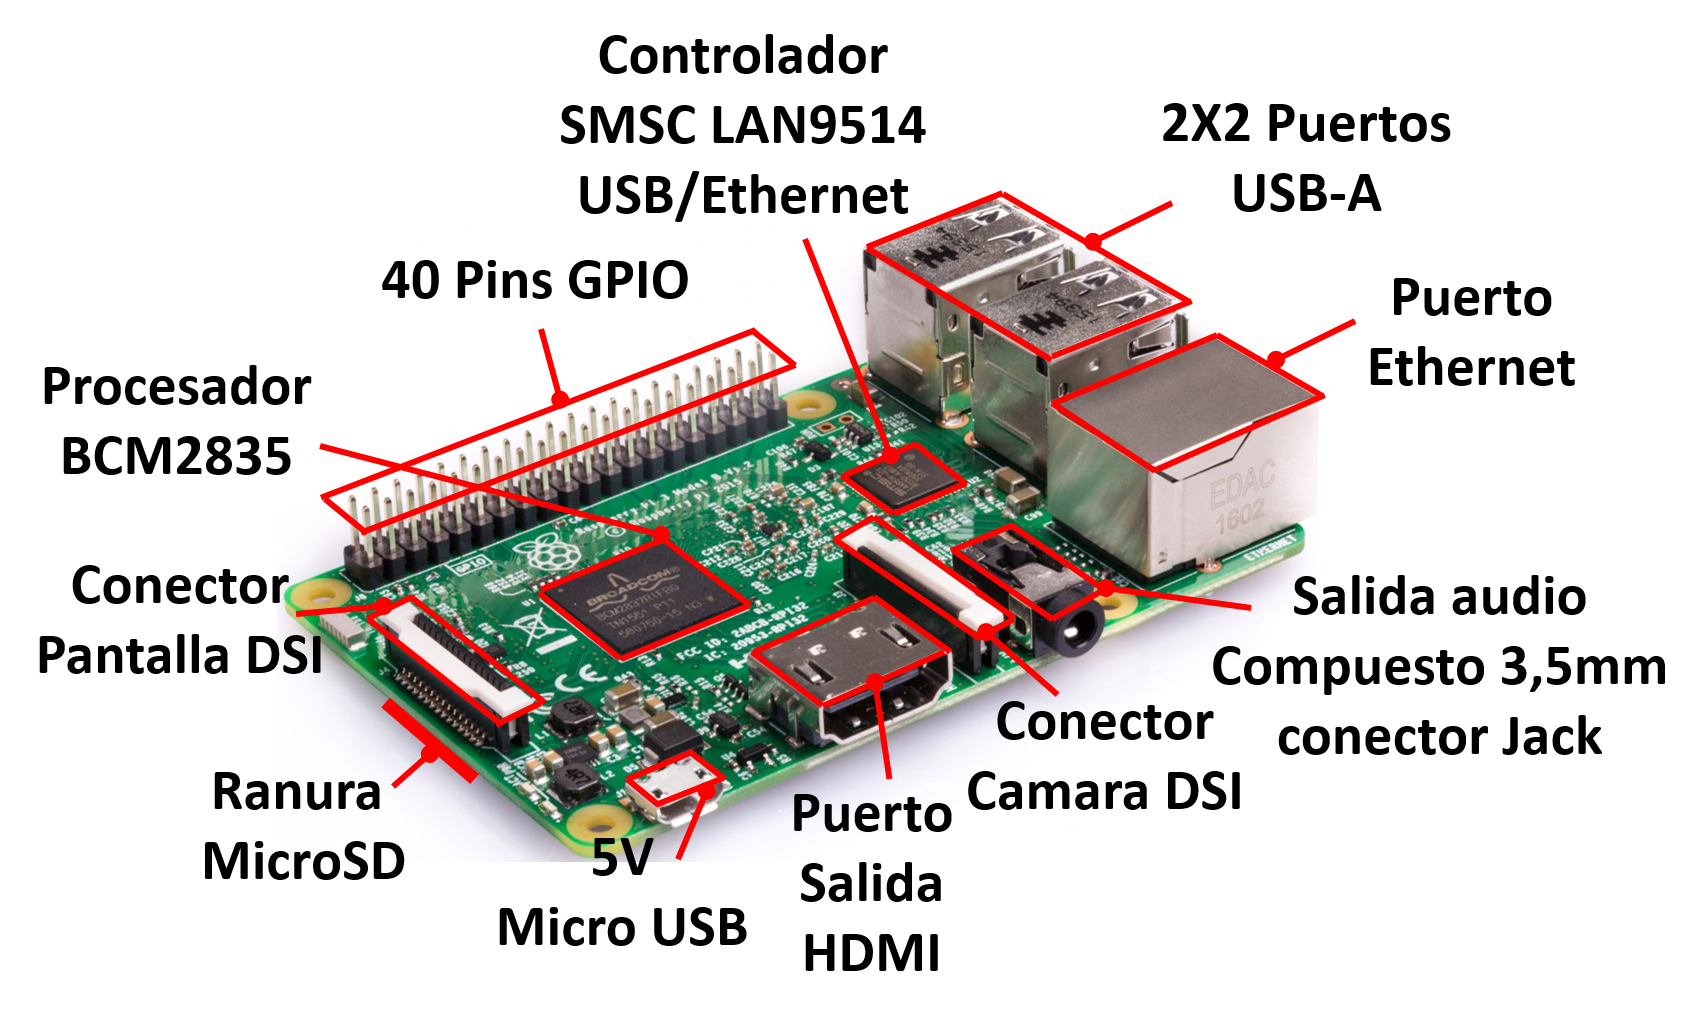
\includegraphics[width=0.7\textwidth]{raspberry3.png}
\caption{Elementos de la laca Raspberry Pi 3B. Fuente: Raspberry Pi User Guide ~\cite{Upton}}
\label{fig:raspberry3}
\end{center}
\end{figure}





\subsection{Pantalla táctil capacitiva.}
\label{subsubs:pantalla7}
En la actualidad, la gran mayoría de los dispositivos comercialmente disponibles, y que hacen uso de una pantalla, usan la tecnología de contacto capacitivo. Estas tecnologías no solo ofrecen un entorno gráfico, sino que también simplifican la interacción \emph{HCI} por el sentido del tacto.\

Las pantallas capacitivas multitáctiles no han sido diseñadas para detectar objetos pasivos al ser situados sobre ellas, estas pantallas incluso disponen de filtros para rechazar de manera activa ese tipo de eventos táctiles.
Los \emph{widgets tangibles} en tales pantallas táctiles capacitivas, se han empezado a explorar relativamente hace poco más de una década\cite{Rekimoto}, pero necesitan generalmente del cuerpo del usuario para proporcionar la capacitancia necesaria para la detección del tacto. La gran limitación es que, para mantener la detección, el usuario tiene que seguir tocando la superficie conductora del \emph{widget}.

Las pantallas táctiles capacitivas, detectan la presencia de un conductor eléctrico conectado a tierra, por lo general un dedo humano, cerca de la superficie de la pantalla que es detectado mediante el uso de electrodos transparentes situados encima de la misma.
Principalmente existen dos técnicas de detección: auto capacitancia y capacitancia mutua~\cite{Barrett}. La capacitancia mutua es el método más comúnmente utilizado en pantallas de tipo multitáctil.\\

La configuración en la que se disponen los electrodos en una pantalla de capacitancia mutua consiste en un conjunto de filas y otro conjunto de columnas. Uno de los conjuntos actúa como transmisores (Tx) y el otro conjunto como receptores (Rx)~\cite{Rekimoto}.

Al aplicar una señal a uno de los electrodos Tx, la capacitancia entre ese electrodo Tx y otro electrodo Rx (que está entrecruzado) acopla la señal al electrodo Rx~\cite{Silicon}. La señal de cada uno de los electrodos Rx es medida y mediante un controlador táctil es determinada la capacitancia entre el electrodo Tx activo y cada uno de los electrodos Rx. Al ser activado un electrodo Tx de manera simultánea (multiplexación en el tiempo), el controlador táctil es capaz de medir esta capacitancia en cada una de las intersecciones de los electrodos Tx - Rx en la pantalla.
Cuando un conductor conectado a tierra como es el caso de un dedo se aproxima a una de estas intersecciones entre electrodos Tx-Rx, la capacitancia entre ambos electrodos se ve reducida cuando el campo eléctrico entre ellos es perturbado por el conductor~\cite{Zimmerman}.

El paso típico de un electrodo es de 5mm, al realizar un toque sobre la pantalla se verán afectadas más de una intersección. El controlador táctil mediante interpolación es capaz de determinar el centro del área tocada e informa de ello con un evento táctil.

La mayor parte de los controladores están diseñados para detectar toques con los dedos, aceptando formas elípticas del tamaño de la yema del dedo y rechazando e ignorando eventos táctiles con otras formas y tamaños que pueden reportar eventos táctiles impredecibles.

Resumiendo, para que el controlador informe de un evento táctil, la capacitancia del electrodo Tx-Rx ha de ser reducida por debajo de cierto umbral y ha de suceder a lo largo una elíptica que forma la yema de un dedo.


\subsubsection{Funcionamiento de un \emph{widget capacitivo}.}

Se define \emph{widget capacitivo} como un objeto tangible completo que contiene uno o más marcadores en su parte inferior y que comunican su posición a la superficie táctil de la pantalla capacitiva. Cada marcador consiste en una almohadilla redonda conductiva que es detectada por la superficie de la pantalla.

Un marcador de \emph{widget} para poder ser detectado como evento táctil sobre la superficie de la pantalla capacitiva, tiene que cumplir el requisito de conexión a tierra. Esto se puede conseguir mediante la capacitancia corporal de un usuario como propone Rekimoto~\cite{Rekimoto}. Esto requiere que el usuario toque el \emph{widget} y que las almohadillas del mismo sean conductivas, además de estar conectadas eléctricamente a la parte del \emph{widget} que es tocada por el usuario. De esta forma el \emph{widget} funciona simplemente como conductor eléctrico entre usuario y superficie táctil. Este enfoque tiene el inconveniente de tan pronto como el usuario deja de tener contacto, el controlador de la pantalla no puede detectar ninguna variación de capacitancia.

Otro enfoque que permite reemplazar al usuario como tierra eléctrica, es el uso de un cable conductor que conecta permanentemente el \emph{widget} a un objeto relativamente conectado a tierra, como es el conector negativo de una batería.

\subsubsection{Pantalla táctil capacitiva HDMI.}
La pantalla multitáctil capacitiva utilizada en la plataforma de juego, y que es incorporada al dispositivo \emph{TUIO1}, es el modelo \emph{7inch HDMI LCD (B)} de la compañía \emph{Waveshare} (ver Figura~\ref{fig:Pantalla7}).

La conexión de la interfaz gráfica con la placa para el desarrollo es tipo \emph{HDMI}, por su compatibilidad y facilidad de uso con \emph{Raspberry Pi}. Los eventos generados en el panel táctil son transmitidos desde el puerto \emph{Micro USB-B} de la propia pantalla, a el puerto \emph{ Micro USB-B} de la placa \emph{Raspberry Pi}.

\begin{figure}[!h]
\begin{center}
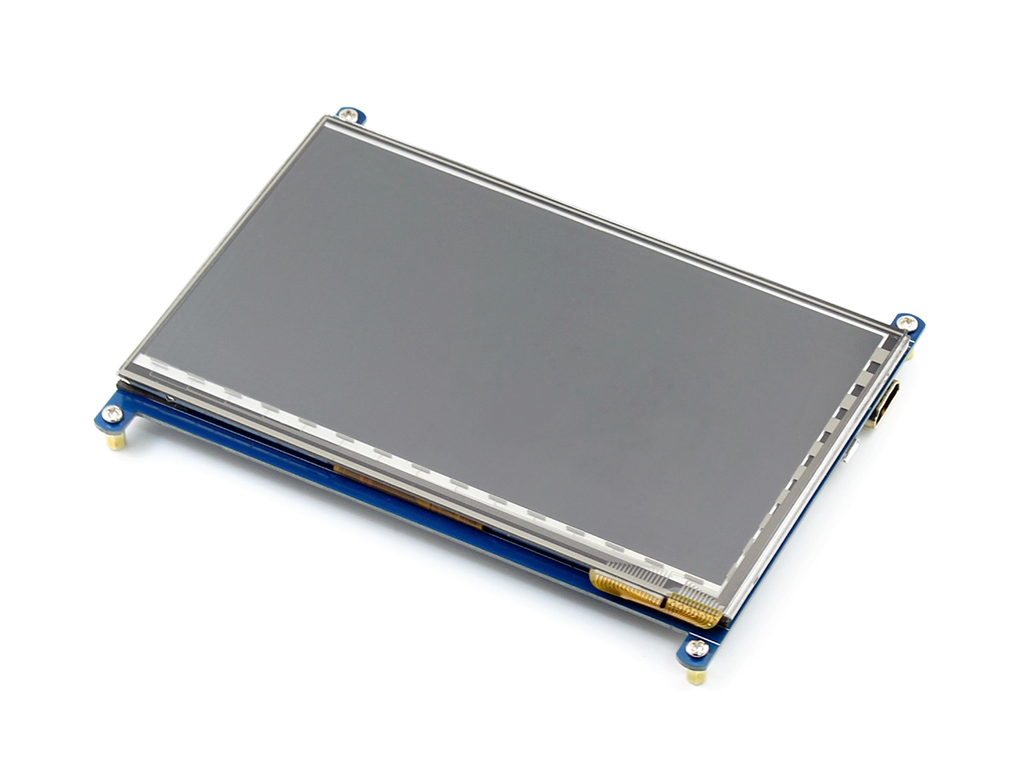
\includegraphics[width=0.7\textwidth]{pantalla7pulgadas.jpg}
\caption{Pantalla táctil capacitiva 7 pulgadas Waveshare. Fuente: Waveshare Electronics ~\cite{Waveshare} }
\label{fig:Pantalla7}
\end{center}
\end{figure}

\textbf{Características principales de la pantalla:}
\begin{itemize}
\item 800x400px alta resolución.
\item Control táctil capacitivo.
\item Interfaz HDMI para la visualización.
\item Interfaz Micro USB-B en el control táctil.
\item Protocolo estándar HID para la integración en el sistema.
\item Soporte para sistemas Raspbian.
\end{itemize}


\textbf{Circuitos y componentes integrados principales para el funcionamiento de la pantalla (Figura~\ref{fig:PropPantalla7}):}
\begin{enumerate}
\item \textbf{Texas Instruments TFP401APZP.} Controlador interfaz digital de pantalla DVI\footnote{Digital Visual Interface}.
\item Atmel AT24MAC602. Memoria EEPROM\footnote{Electrically Erasable Programmable Read-Only Memory}.
\item Goodix GT811. Controlador interfaz panel táctil.
\item ST Microelectronics STM32F103. Procesador ARM 32-bit Cortex-M3 CPU core.
\item AMS1117. Regulador de voltaje.
\item Conector FFC\footnote{Flexible Flat Cable} panel táctil .
\item Conector FCC pantalla.
\item Puerto HDMI.
\item Puerto Micro USB-B.
\item Micro interruptor de luz de fondo.
\end{enumerate}

\begin{figure}[!h]
\begin{center}
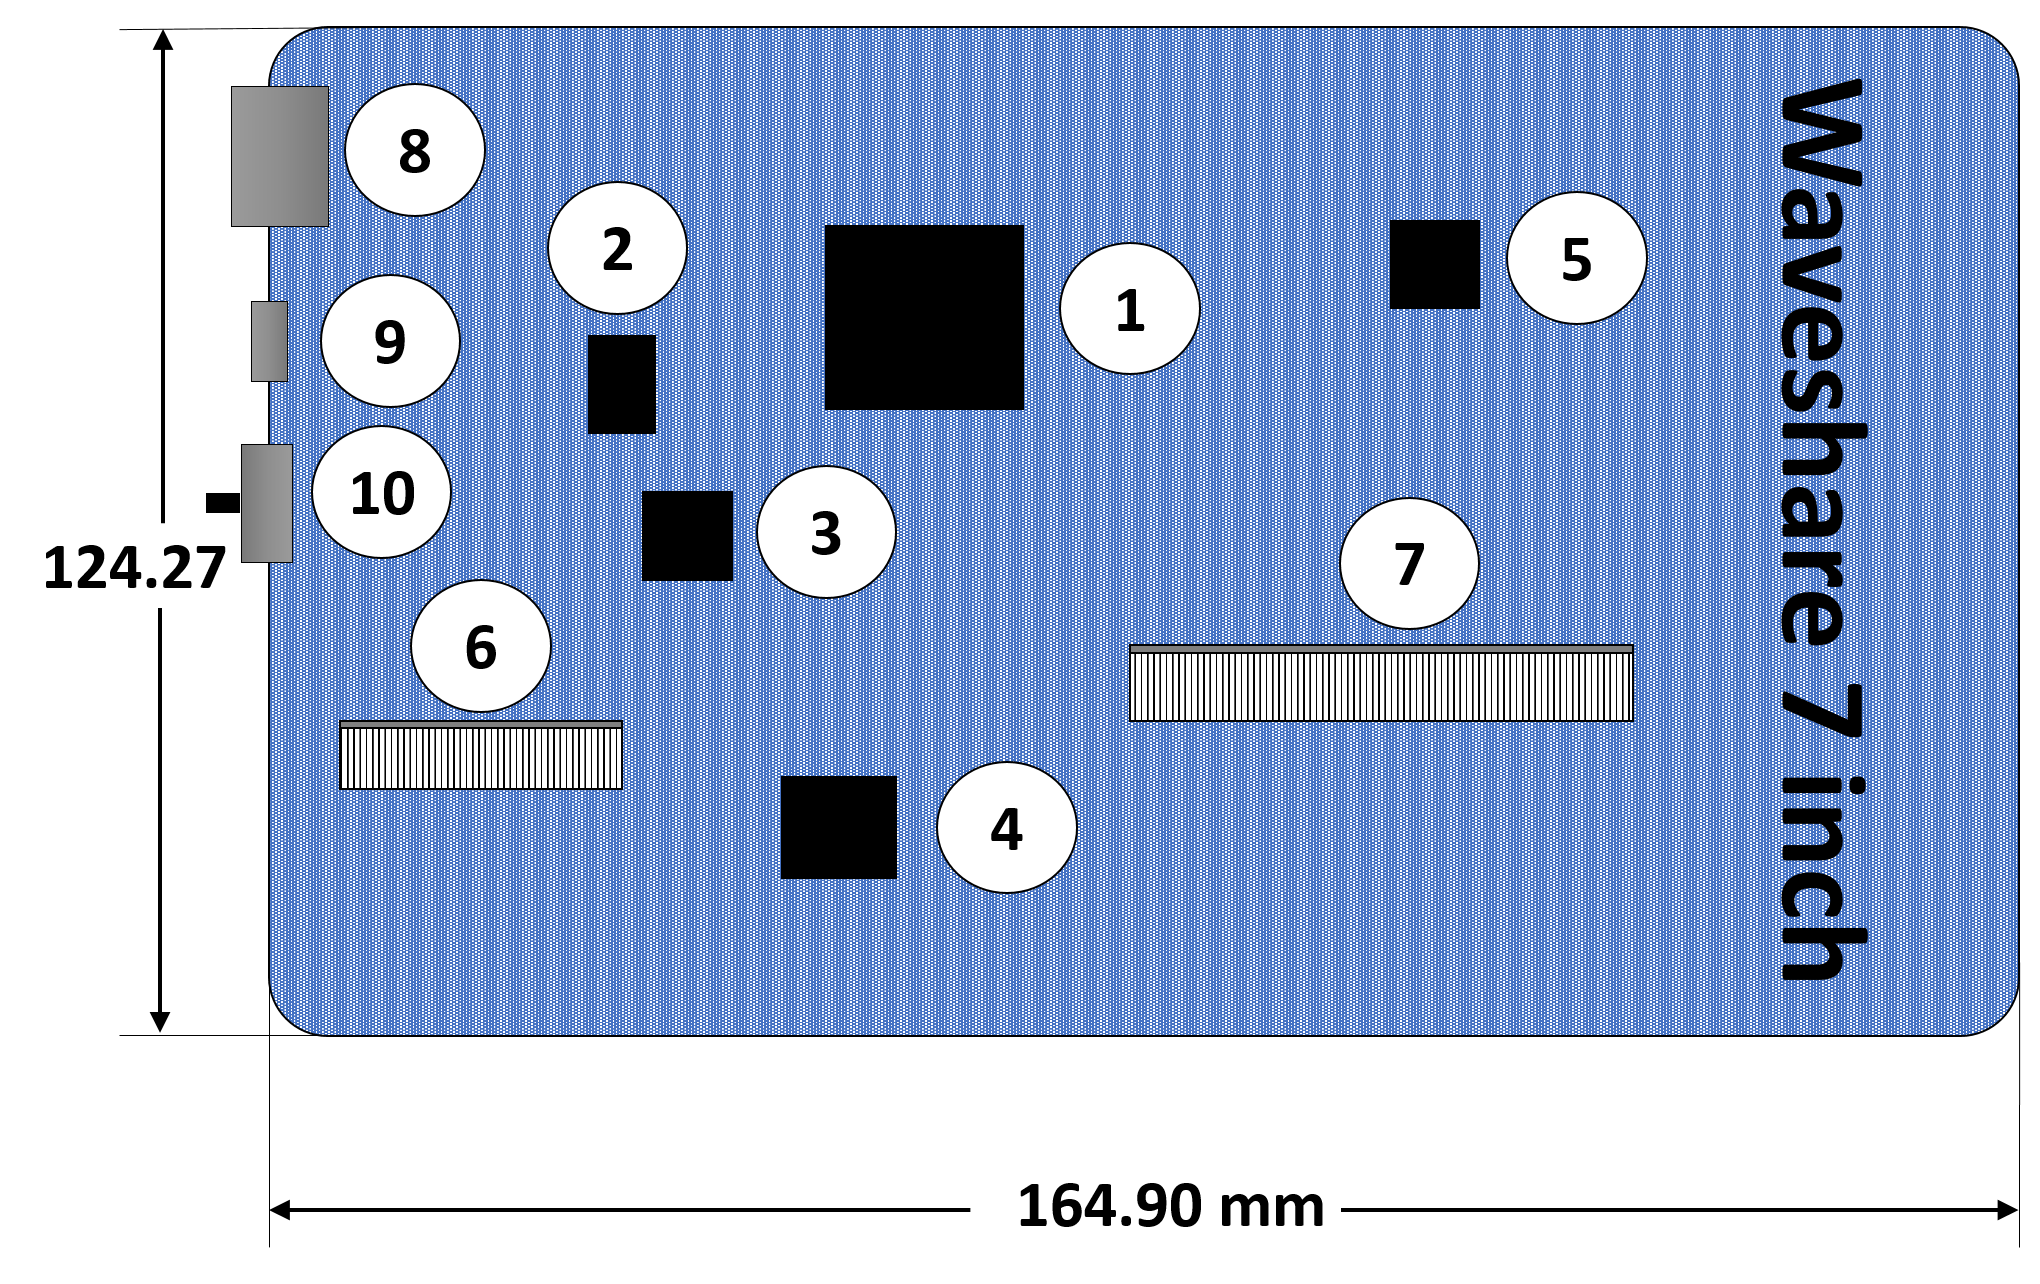
\includegraphics[width=0.8\textwidth]{pantallaTUIO1.png}
\caption{Componentes panel táctil capacitivo 7 pulgadas.}
\label{fig:PropPantalla7}
\end{center}
\end{figure}

\subsubsection{Instalación de los controladores de la pantalla en Raspbian.}

La instalación de los \emph{drivers} dentro del sistema operativo \emph{Raspbian}, se realiza por línea de comandos, ejecutando los siguientes pasos:\\
Obtener la última versión de los controladores desde el repositorio Git.\\
\colorbox[gray]{0.85}{\texttt{git clone https://github.com/goodtft/LCD-show.git}}\\
Cambiar los permisos de lectura, escritura y ejecución de \texttt{LCD-show} y entrar al directorio.\\
\colorbox[gray]{0.85}{\texttt{chmod -R 755 LCD-show}}\\
\colorbox[gray]{0.85}{\texttt{cd LCD-show/}}\\
Ejecutar la instalación de los drivers, en este caso, la version B de la pantalla 7.0 pulgadas.\\
\colorbox[gray]{0.85}{\texttt{sudo ./LCD7B-show}}\\
Después de reiniciar el sistema, la pantalla puede ser utilizada en Raspbian.

Las características y proceso de configuración, han sido obtenidos de \textbf{ Waveshare Electronics ~\cite{Waveshare}}


\subsection{Pantalla táctil resistiva HDMI.}
\label{subsubs:pantalla3}
Una pantalla táctil resistiva está formada por un panel de vidrio o acrílico, recubierto con dos capas eléctricamente conductoras y resistivas, con una separación entre ambas, y fabricadas con óxido de indio y estaño. Estas capas al ser presionadas producen un cambio en su resistencia. La producción de ente tipo de tecnología es más económico que el tipo capacitivo, con el inconveniente de solo detectar un evento táctil simultáneo ~\cite{Downs}.

La pantalla resistiva utilizada en la plataforma de juego, y que es incorporada al dispositivo \emph{TUIO2}, es el modelo \emph{3.5inch HDMI LCD} de la compañía \emph{Kedei}(ver Figura~\ref{fig:Pantalla7}).

La conexión de la interfaz gráfica con la placa para el desarrollo es \emph{HDMI}, por su compatibilidad y facilidad de uso con \emph{Raspberry Pi}. Los eventos generados en el panel táctil son transmitidos a la placa por comunicación \emph{SPI}.

\textbf{Características principales de la pantalla:}
\begin{itemize}
\item 480x320px alta resolución.
\item Control táctil resistivo.
\item Interfaz HDMI para la visualización.
\item Interfaz SPI en el control táctil.
\item Protocolo estandar HID para la integración en el sistema.
\item Soporte para sistemas Raspbian.
\end{itemize}

\begin{figure}[!h]
\begin{center}
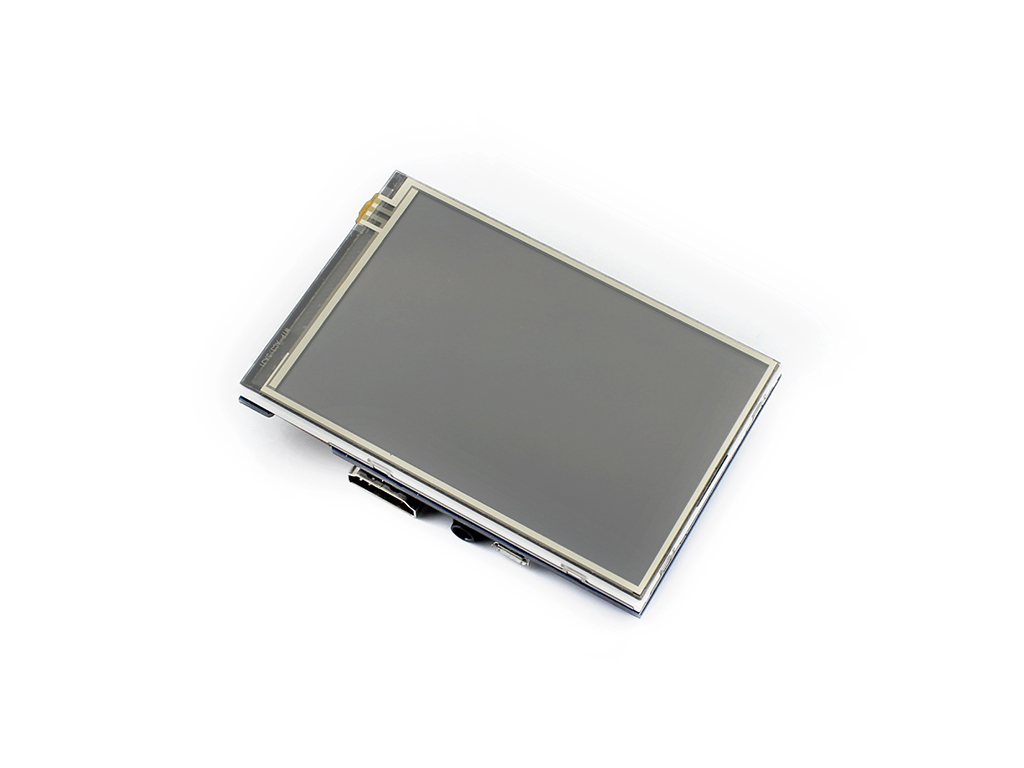
\includegraphics[width=0.8\textwidth]{pantalla3pulgadas.jpg}
\caption{Componentes pantalla táctil capacitiva 3.5 pulgadas}
\label{fig:Pantalla3}
\end{center}
\end{figure}

\textbf{Circuitos y componentes integrados principales, para el funcionamiento de la pantalla (Figura~\ref{fig:ProPantalla3}):
}
\begin{figure}[!h]
\begin{center}
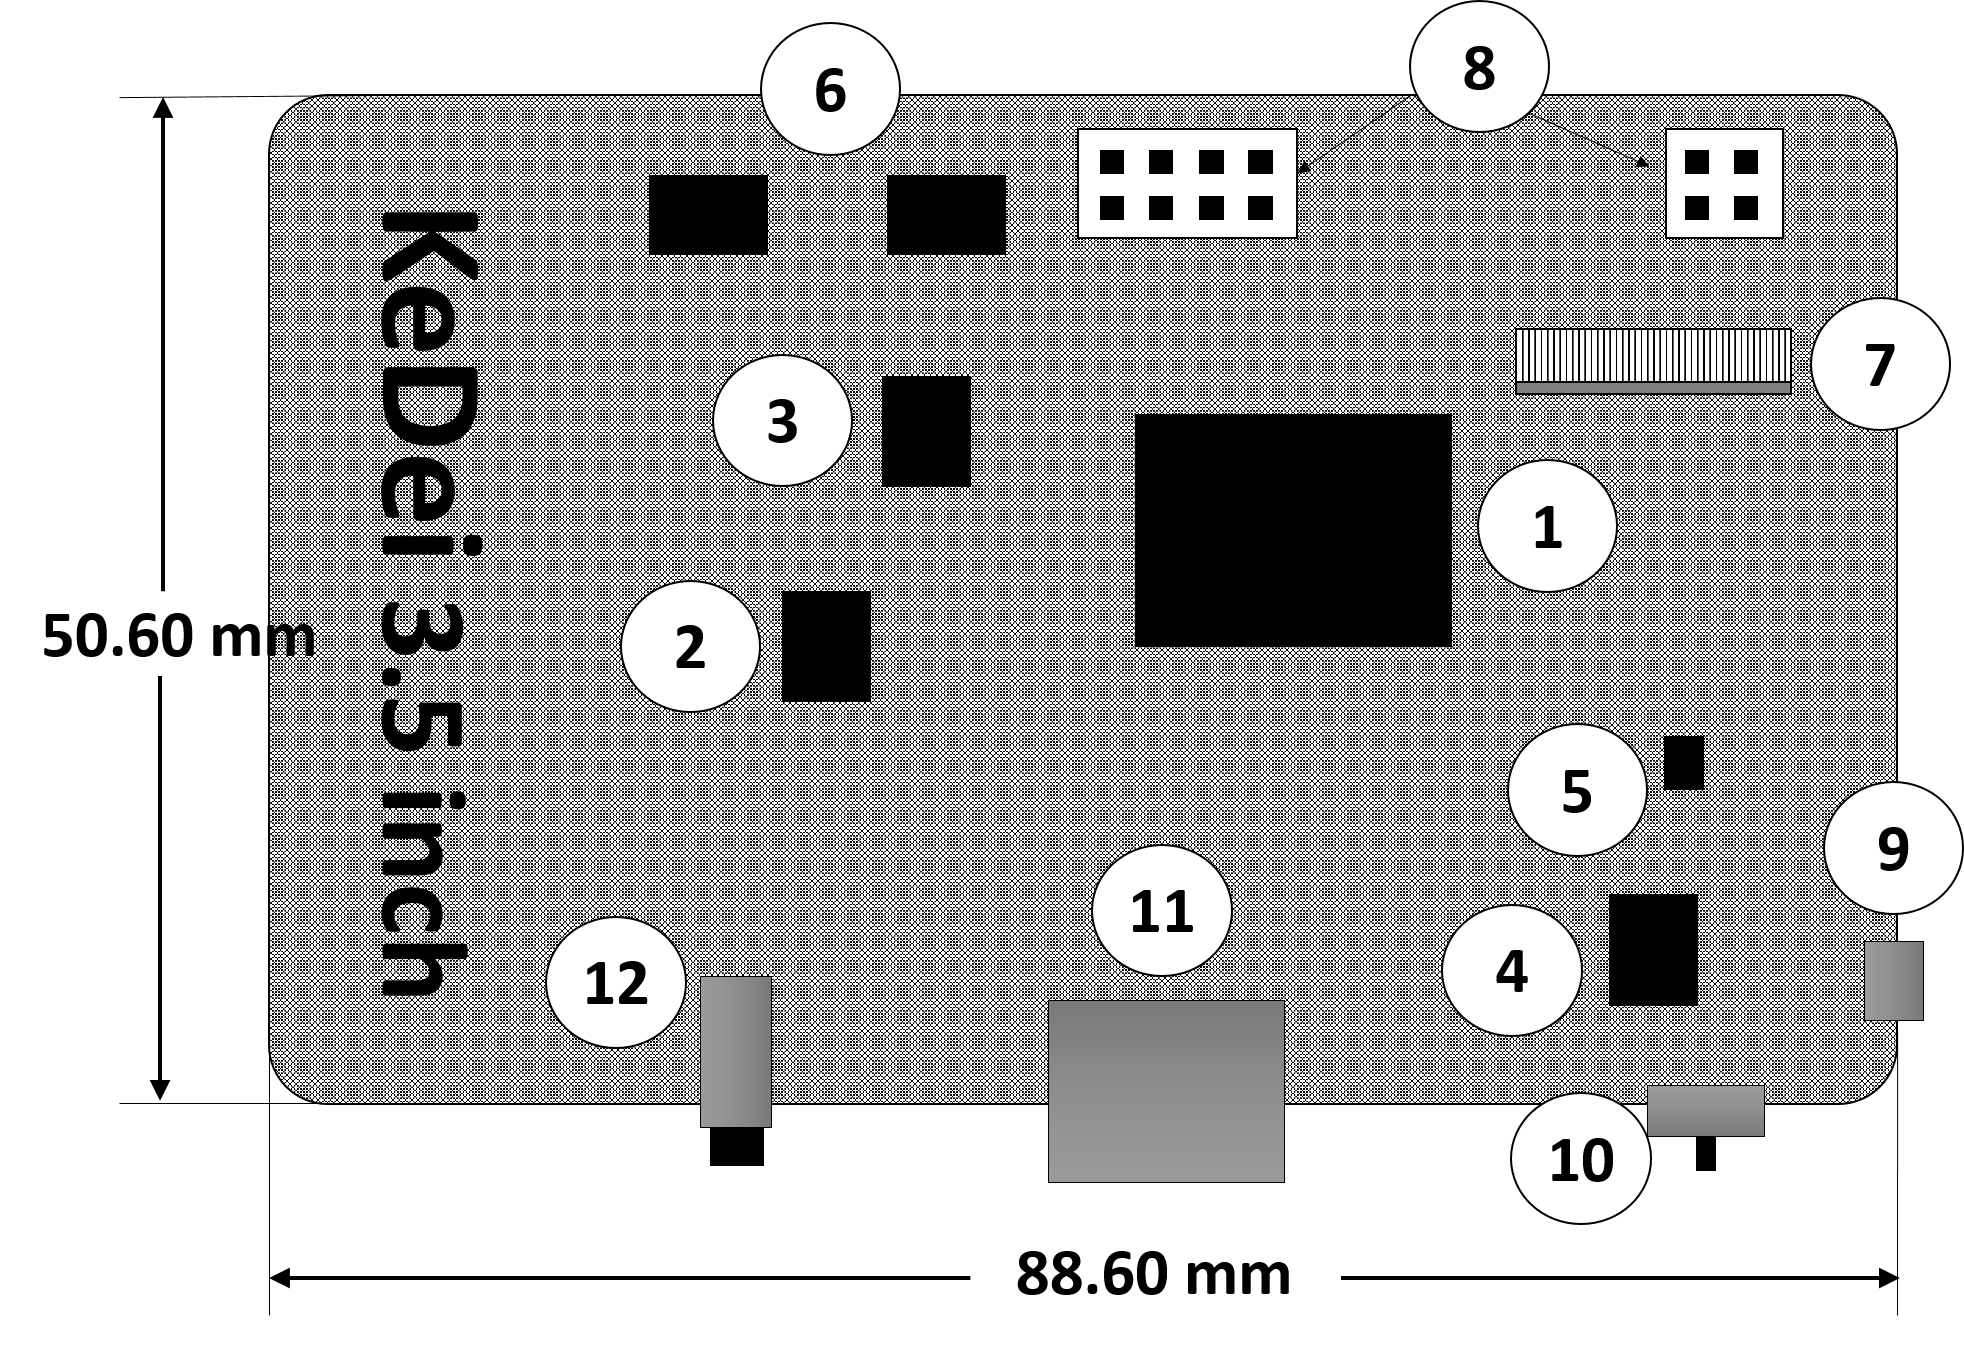
\includegraphics[width=0.65\textwidth]{pantallaTUIO2.png}
\caption{Componentes pantalla táctil capacitiva 3.5 pulgadas}
\label{fig:ProPantalla3}
\end{center}
\end{figure}

\begin{enumerate}
\item \textbf{Realtek RTD2660H.} Controlador interfaz digital de pantalla.
\item \textbf{Winbond W25X40CLNIG.} Memoria Flash 4Mbit SPI.
\item \textbf{Cirrus Logic CS4334.} Convertido estéreo D/A 24bit 96kHz con interfaz I2S.
\item \textbf{Shenzhen Xptek Technology XPT2046.} Controlador interfaz panel táctil con interfaz I2C.
\item \textbf{PowerTech PT4103.} Controlador para leds por ancho de pulsos PWM \footnote{pulse width modulation}. 
\item \textbf{AMS1117.} Regulador de voltaje.
\item Conector FCC pantalla.
\item Conector GPIO (Alimentación y panel táctil).
\item Puerto Micro USB-B.
\item Interruptor de luz de fondo.
\item Puerto HDMI.
\item Puerto salida de audio.
\end{enumerate}

\subsubsection{Instalación de los controladores de la pantalla en Raspbian.}
El primer paso para la instalación de los \emph{drivers}, es descargar la última versión en la dirección: \emph{http://osoyoo.com/driver/LCD\_show\_35hdmi.tar.gz}.\\
Desde el directorio de descarga, y por medio de línea de comandos, se cambian los permisos de ejecución:\\
\colorbox[gray]{0.85}{\texttt{sudo chmod 777 LCD\_show\_35hdmi.tar.gz}}\\
Descomprimir el archivo y entrar dentro de la carpeta donde se encuentran los controladores:\\
\colorbox[gray]{0.85}{\texttt{tar -xzvf LCD\_show\_35hdmi.tar.gz}}\\
\colorbox[gray]{0.85}{\texttt{cd LCD\_show\_35hdmi}}\\
Instalar el controlador adecuado para la resolución de la pantalla (480x320):\\
\colorbox[gray]{0.85}{\texttt{sudo ./LCD35\_480*320}}\\
Después de reiniciar automáticamente el sistema, la pantalla puede ser utilizada en \emph{Raspbian}.



\subsection{Dispositivos de entrada. Sensores.}
Un sensor es un dispositivo que, a partir de la energía del medio donde se mide, da una señal de salida transducible, que es función de la variable medida. Es decir, un sensor es capaz de convertir una señal mecánica, a una señal de tipo eléctrico ~\cite{Payas}. 



\subsubsection{Unidad de medición inercial MPU9255.}

Definimos un sensor inercial como aquel que es usado para medir las variaciones de velocidad lineal, angular y campo magnético, producidas en una masa.
Un sensor inercial por tanto dispone de tres transductores de señal: acelerómetro (medidas de velocidad lineal), giróscopo (medición de velocidad angular), y magnetómetro (medidas de la variación del campo magnético).

Habitualmente son utilizados como componentes fundamentales en sistemas de navegación donde es necesario estimar mediciones de posición, posición y velocidad de un cuerpo, en ausencia de referencias externas.

La unidad de medición inercial utilizada es \emph{MPU9255} de la compañía \emph{InvenSense}. Este dispositivo electrónico es la combinación de dos sensores, \emph{MPU-6500} y \emph{AK8963}. El sensor \emph{MPU-6500} contiene un giroscopio de tres ejes y un acelerómetro de tres ejes, capaz de tomar mediciones de aceleraciones y velocidades angulares, de un cuerpo al que este fijado. Está complementado con un procesador digital de movimiento \emph{DMP}\footnote{Data Management Platform}. \emph{AK8963} es un sensor de medición del campo magnético gravitacional (magnetómetro) digital. La comunicación con los registros del dispositivo se realiza utilizando el bus de datos \emph{I2C} a 400kHz.\\

\textbf{Especificaciones generales del MPU9255:}
\begin{itemize}
\item Voltaje de operación (VDD): 2.4V – 3.6V
\item Voltaje de interfaz digital (VDDIO): 1.71V – VDD
\item Rango de temperatura: -40ºC – 85ºC
\item Frecuencia de operación I2C: 400kHz
\item Bus auxiliar I2C maestro para leer datos de sensores externos (p. Ej. Sensor de presión).
\item Corriente de operación de 3.5mA cuando los 9 ejes de detección de movimiento y el DMP están habilitados.
\item Rango de voltaje VDD: 2.4 - 3.6V.
\item Voltaje de referencia VDDIO para dispositivos I2C auxiliares.
\item Memoria intermedia FIFO de 512 bytes que permite al procesador leer los datos en ráfagas.
\item Sensor de temperatura de salida digital.
\item Filtros digitales programables por el usuario para giroscopio, acelerómetro y sensor de temperatura
\end{itemize}


\textbf{Características del giroscopio:}
\begin{itemize}
\item Sensores de velocidad angular ejes X, Y y Z de salida digital con un rango de escala completa programable por el usuario de \emph{$\pm 250, \pm 500, \pm 1000, \pm 2000  {\circ}/seg$} y controladores integrados de 16 bits.
\item Filtro de paso bajo programable digitalmente.
\item Corriente de funcionamiento: 3.2mA.
\item Modo de reposo: $8\mu A$.
\end{itemize}


\textbf{Características del acelerómetro:}
\begin{itemize}
\item Acelerómetro de triple eje, salida digital con un rango programable de escala completa de \emph{$\pm 2 g , \pm 4 g , \pm 8 gy \pm 16 g$} y ADC integrado de 16 bits.
\item Corriente de funcionamiento normal del acelerómetro: $450 \mu A$.
\item Corriente del modo acelerómetro de baja potencia: $8.4\mu A$ a 0.98Hz, $19.8\mu A$ a 31.25Hz.
\item Modo de reposo: $8\mu A$
\end{itemize}

\textbf{Características del magnetómetro:}
\begin{itemize}
\item Sensor magnético de \emph{efecto Hall} monolítico de silicio de 3 ejes con concentrador magnético.
\item Resolución de datos de salida de 14 bit ($0.6\mu T / LSB$) o 16 bit ($15\mu T / LSB$).
\item El rango de medición a escala completa es de  $4800\mu T$.
\item Corriente de funcionamiento normal del magnetómetro: $280\mu A$ a una frecuencia de repetición de 8Hz.
\end{itemize}


El sensor permite comunicarse por dos buses distintos: \emph{I2C} y \emph{SPI}. El dispositivo \emph{TUIO2} emplea las comunicaciones \emph{SPI} con la interfaz del panel táctil, por lo que para simplificar se emplea las comunicaciones \emph{I2C}.\\

\textbf{Descripción de las señales y pines de salida para una configuración I2C(Figura~\ref{fig:MPU9255_PINS} y Figura~\ref{fig:MPU9255_I2C}):}
\begin{enumerate}
\item \textbf{VCC:} Entrada voltaje positivo fuente de alimentación del circuito.
\item \textbf{GND:} Terminal negativo de la fuente de voltaje de alimentación.
\item \textbf{SCL:} Señal de reloj serie I2C.
\item \textbf{SDA:} Entrada de datos serie I2C.
\item \textbf{nCS:} Selector de chip (solo para comunicaciones SPI).
\item \textbf{AD0:} Dirección esclavo I2C.
\item \textbf{INT:} Entrada interrumpir suspensión del sistema.
\item \textbf{FSYNC:} Entrada digital de sincronización de \emph{frames}.
\item \textbf{AUX-CL:} Señal de reloj I2C para conectar sensores externos al dispositivo.
\item \textbf{AUX-DA:} Señal de entrada de datos serie I2C, para conexiones de sensores externos. 
\end{enumerate}

\begin{figure}[!h]
\begin{center}
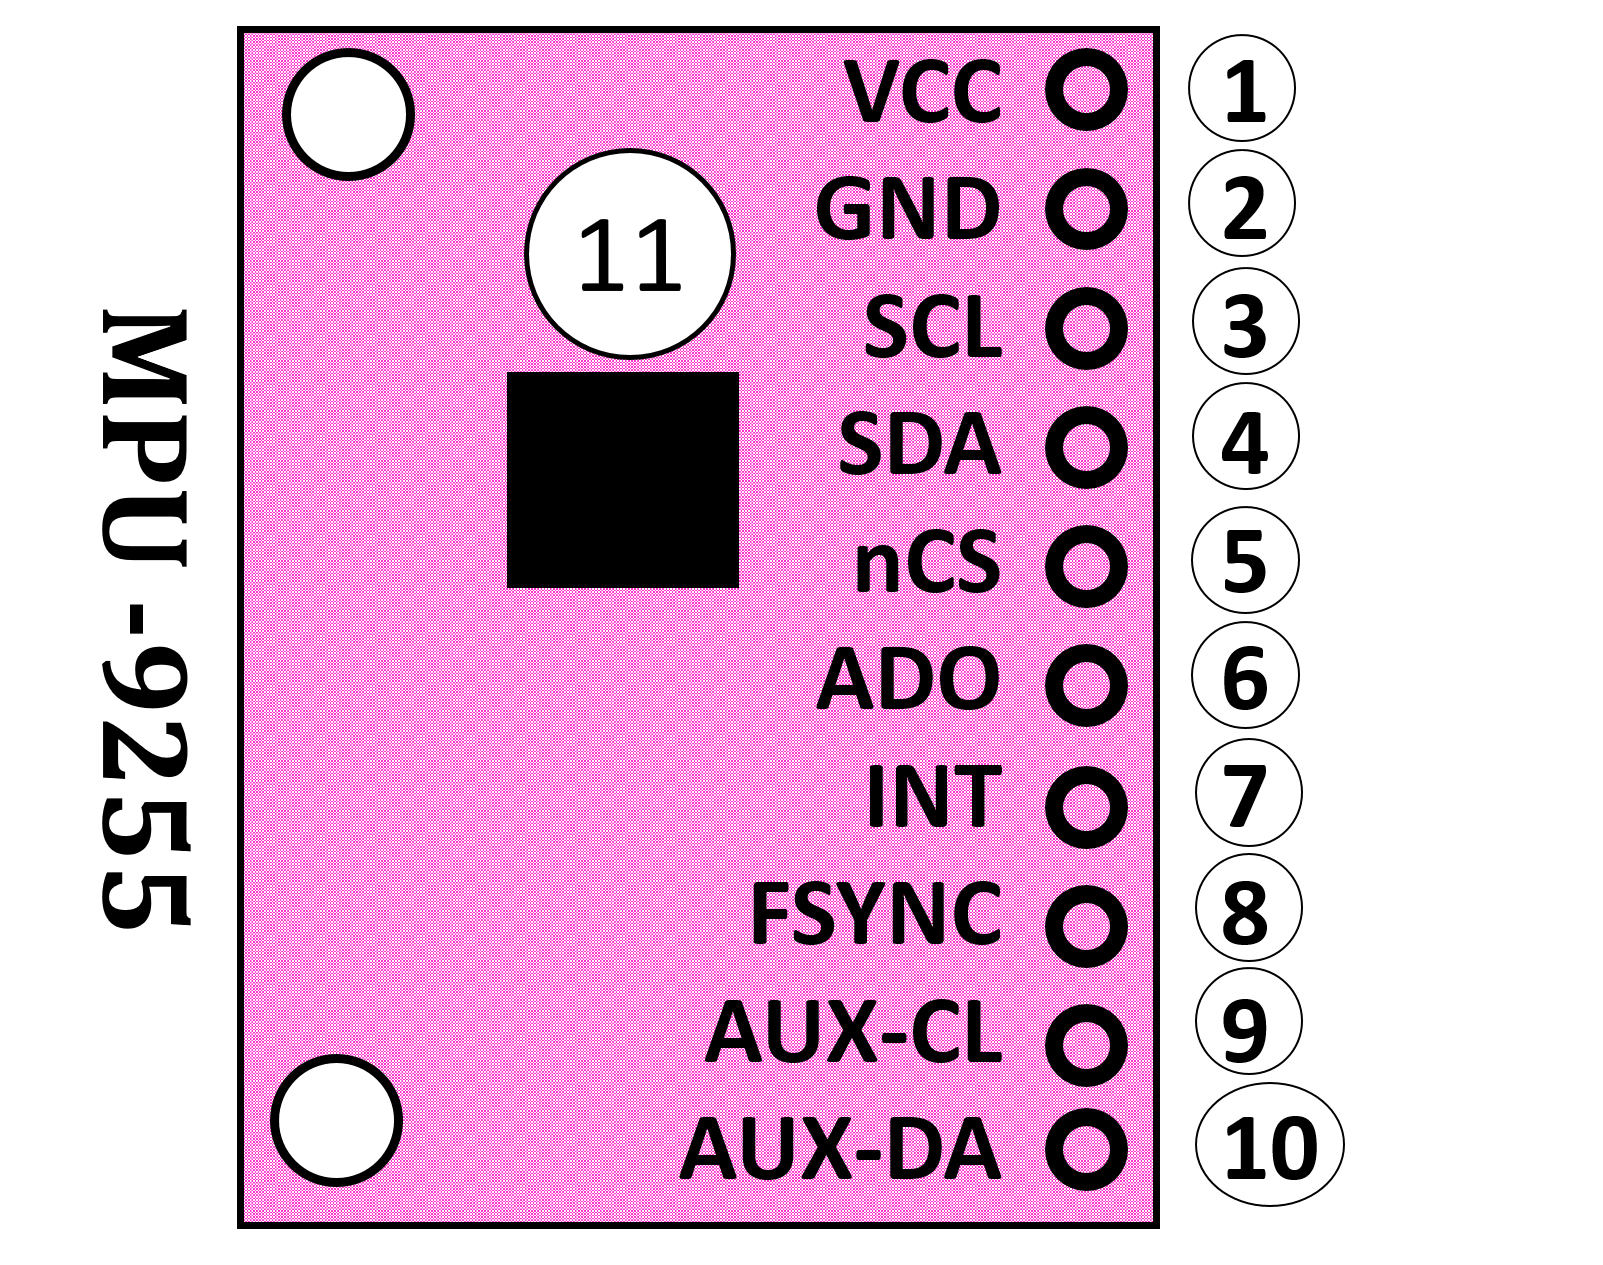
\includegraphics[width=0.4\textwidth]{MPU9255_PINS.png}
\caption{Pines de la unidad de medición inercial MPU9255.}
\label{fig:MPU9255_PINS}
\end{center}
\end{figure}

\begin{figure}[!h]
\begin{center}
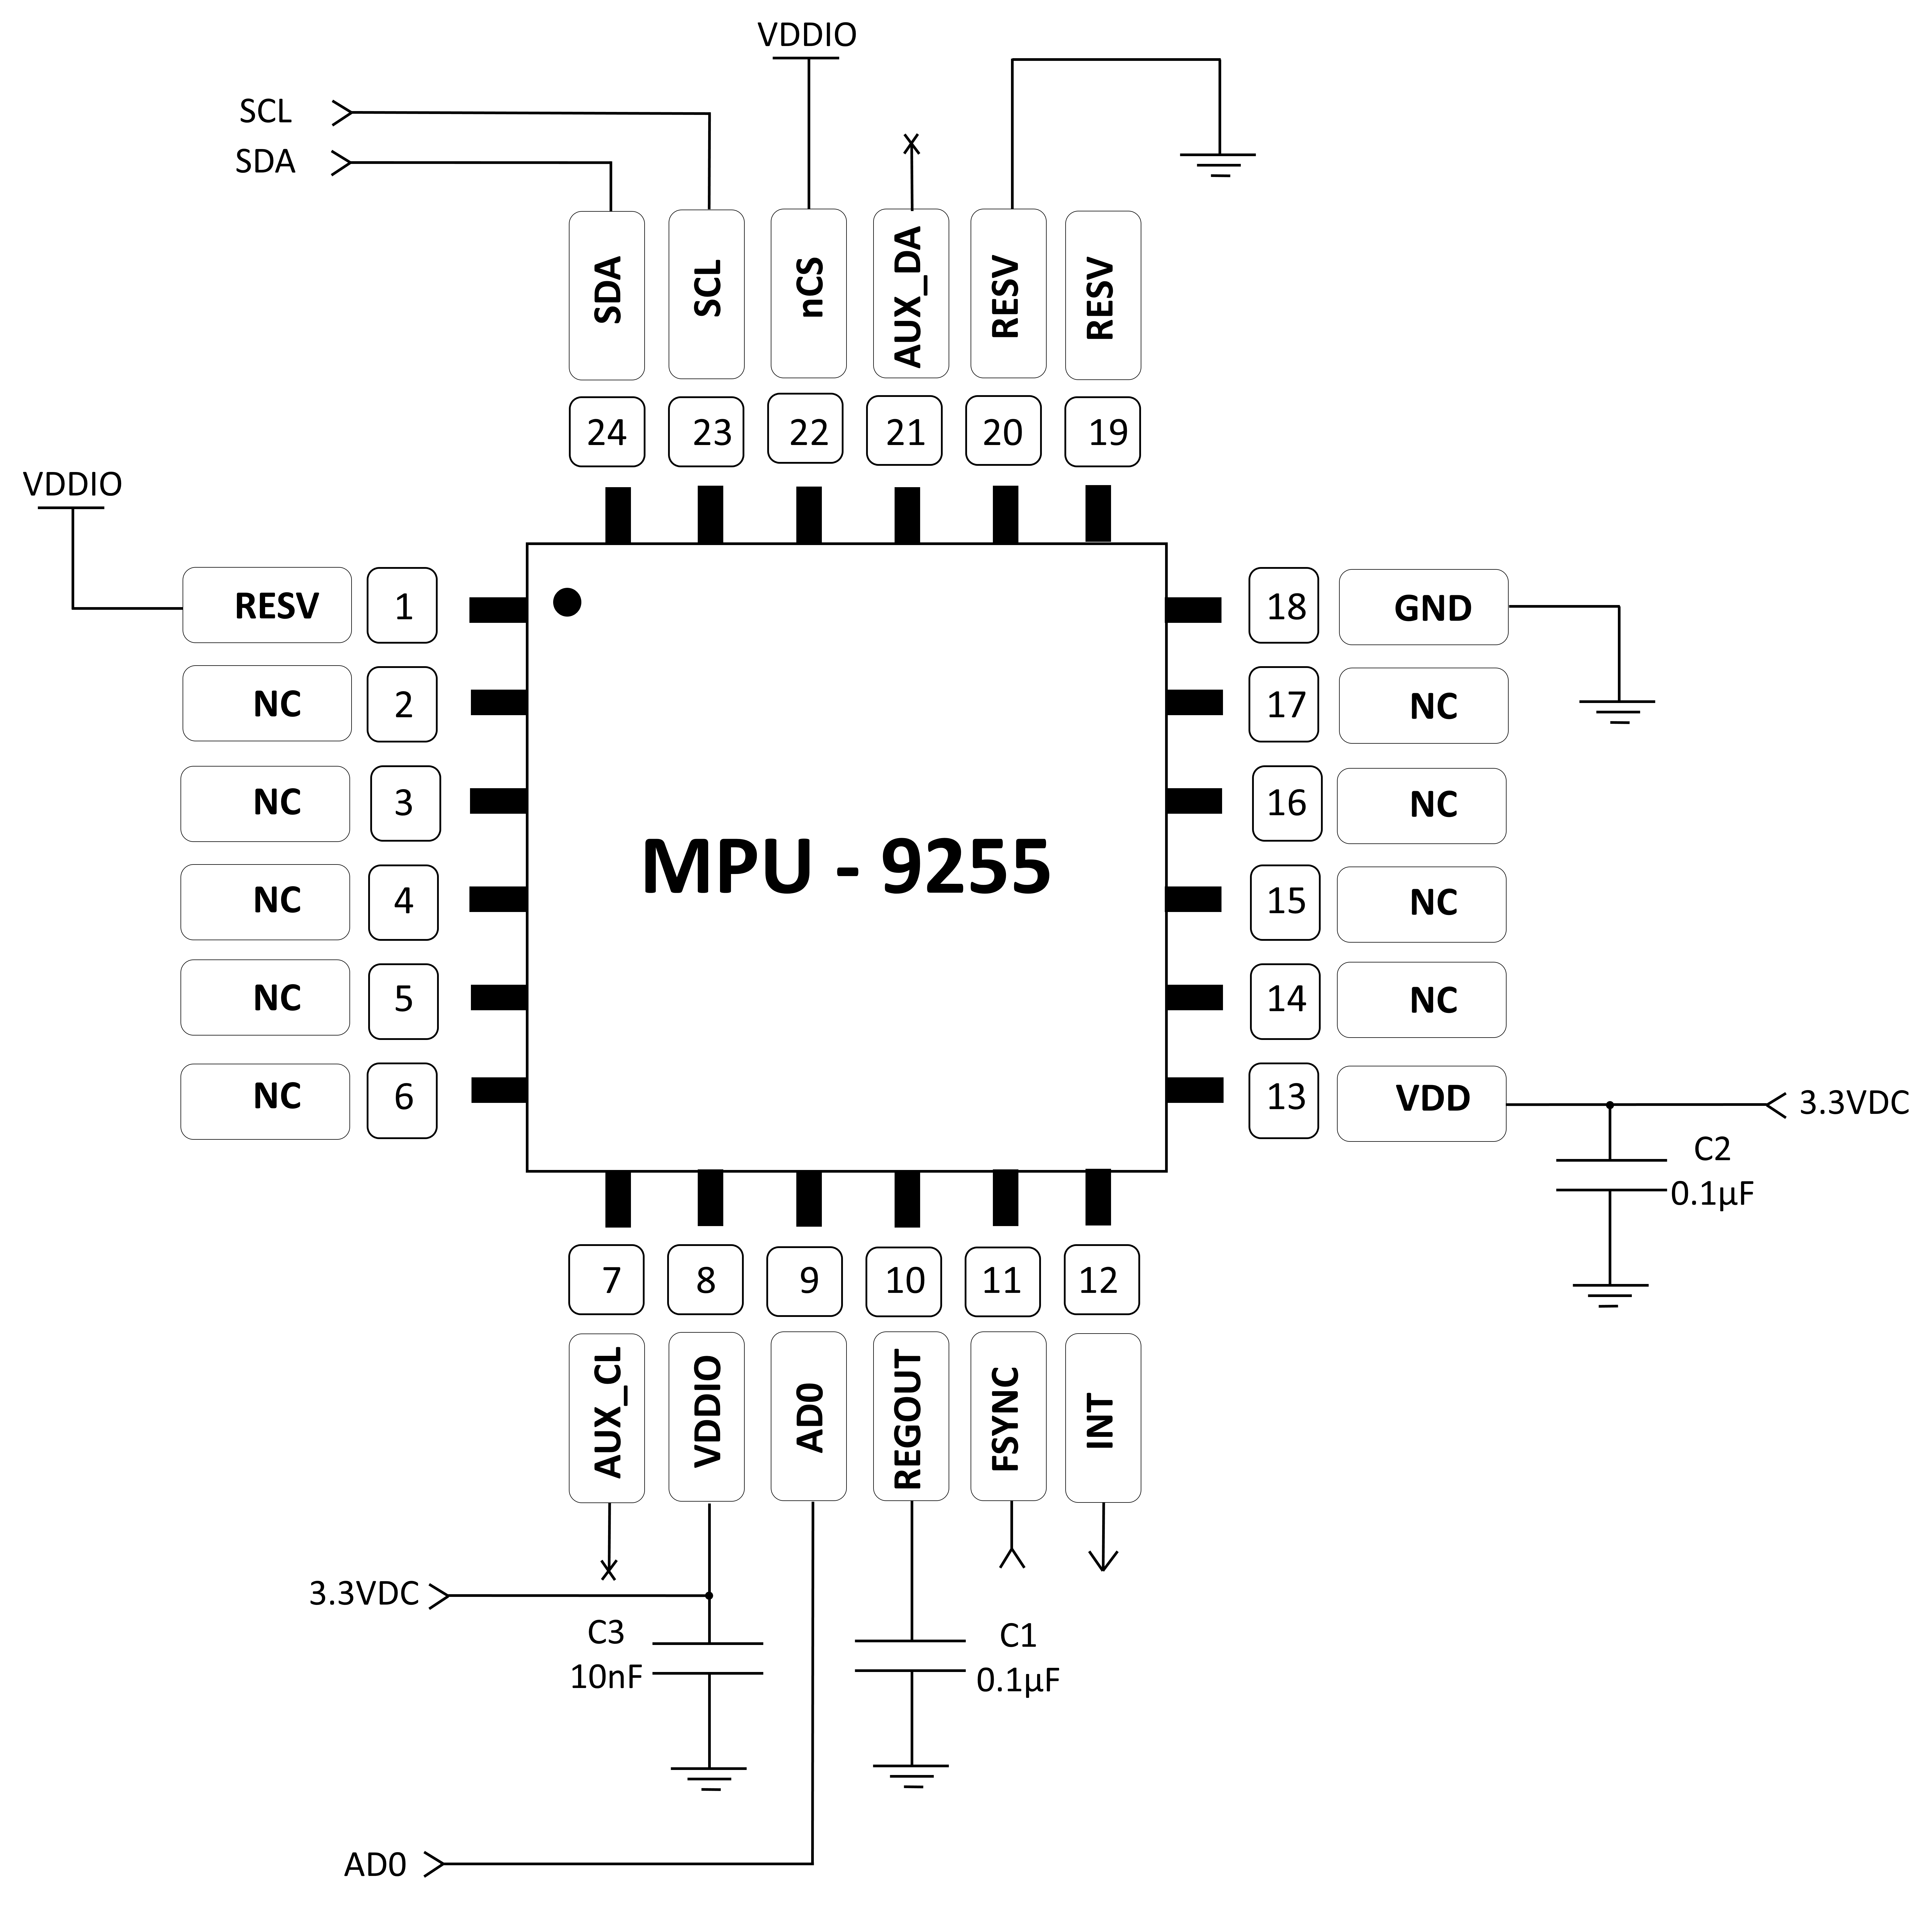
\includegraphics[width=0.75\textwidth]{MPU9255_I2C.png}
\caption{Esquema para una aplicación con bus I2C en MPU9255.}
\label{fig:MPU9255_I2C}
\end{center}
\end{figure}

La conexión con la placa para el desarrollo \emph{Raspberry Pi} para comunicaciones \emph{I2C}, se realiza mediante 4 líneas (ver Figura~\ref{fig:MPU9255_I2C}).

\begin{figure}[!h]
\begin{center}
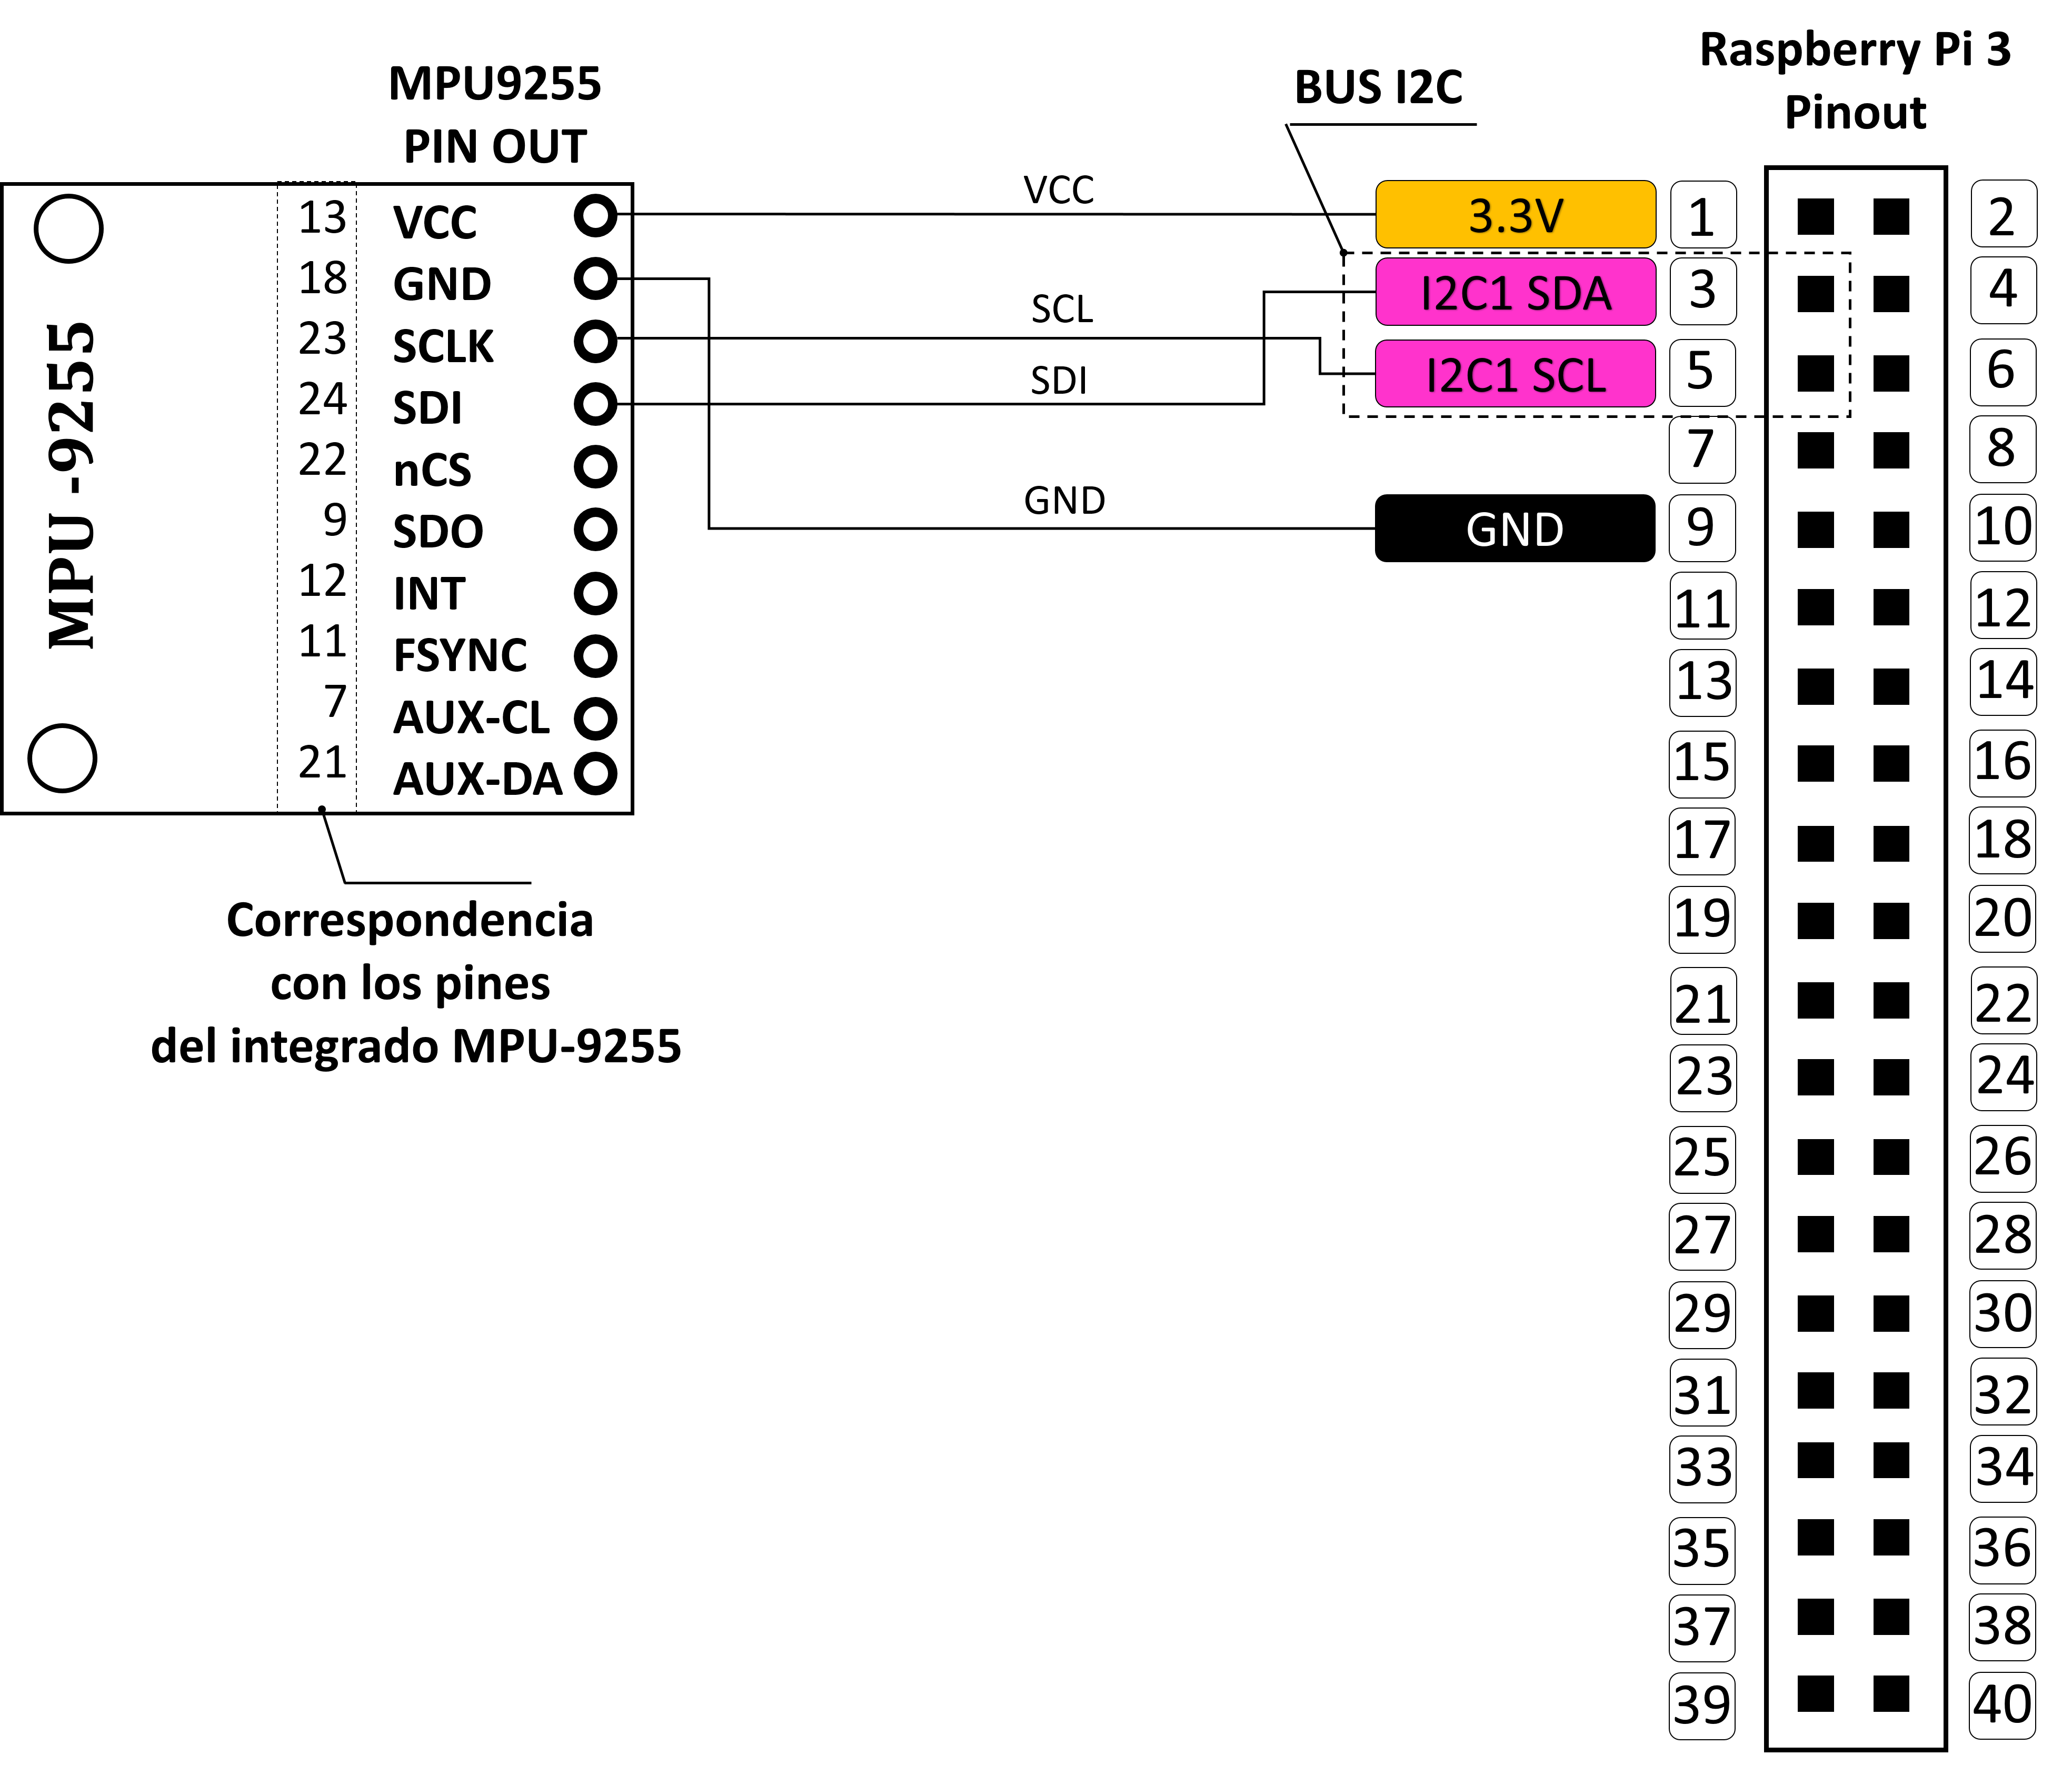
\includegraphics[width=0.8\textwidth]{MPU9255_PINOUT.png}
\caption{Esquema de conexiones con Raspberry Pi para comunicaciones I2C.}
\label{fig:MPU9255_PINOUT}
\end{center}
\end{figure}

Los datos técnicos, así como la descripción de sus componentes, han sido obtenidos de la documentación facilitada por el fabricante ~\cite{MPU9255}.


\subsubsection{Sensor de color.}





\section{Software para el desarrollo.}
\label{sec:software}

\subsection{Sistema Operativo GNU/Linux. Raspbian.}
\label{subs:raspbian}
\emph{GNU/Linux} es un sistema operativo que utiliza el \emph{Kernel Linux} como núcleo. Fue creado y difundido, a través del Proyecto \emph{GNU} por la \emph{Free Software Foundation}, fundada por Richard Stallman, uno de los principales percusores del Software Libre .
Las distribuciones basadas en el Kernel Linux, destacan: \emph{Ubuntu, Kubuntu, Fedora, ArchLinux, Debian}, entre otros ~\cite{Upton}. 
\emph{Raspbian} es un sistema operativo basado en la distribución \emph{Debian}, recomendado para \emph{Raspberry Pi} por estar optimizado para su hardware, siendo la más estable y con mayor rendimiento. Dispone de conjuntos de paquetes (por defecto incorpora más de 35000 paquetes) con fines específicos para este tipo de dispositivos ~\cite{Upton}.

\begin{figure}[!h]
\begin{center}

\includegraphics[width=0.3\textwidth]{debianlogo.jpg}
\caption{Logotipo Raspbian/Debian. Fuente: Página Oficial Raspberry Pi ~\cite{Raspberry}.}
\label{fig:MPU9255_PINOUT}
\end{center}
\end{figure}

\subsubsection{Instalación de Raspbian}
Para instalar el sistema operativo Raspbian, es necesario descargar y descomprimir en una tarjeta microSD (con formato VFAT), la versión de NOOBS 1.9 desde la página oficial de \emph{Raspberry Pi Foundation ~\cite{Noobs}}.
Al realizar el primer arranque, el menú de NOOBS (Figura ~\ref{fig:noobs} instala de manera automática \emph{Raspbian}.
\begin{figure}[!h]
\begin{center}
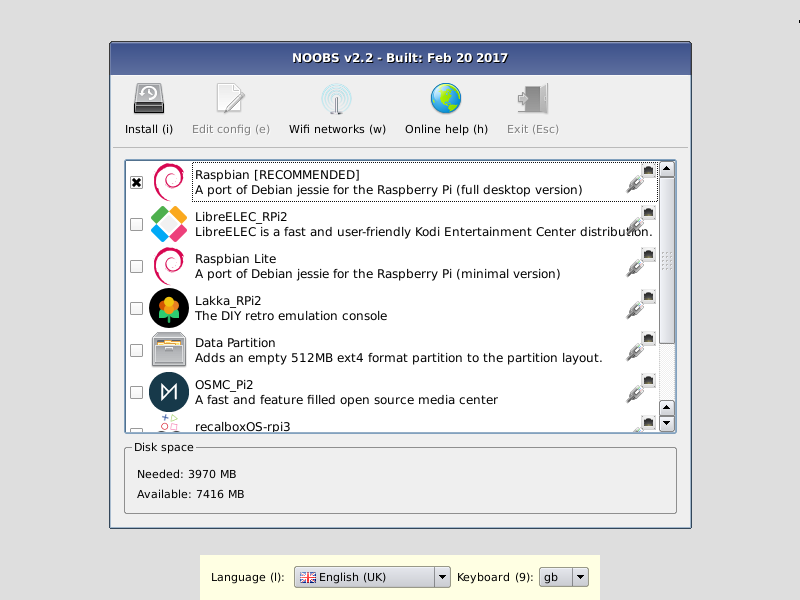
\includegraphics[width=0.7\textwidth]{noobs.png}
\caption{Menú de instalación NOOBS.}
\label{fig:noobs}
\end{center}
\end{figure}
Al reiniciar, el sistema entra automáticamente en modo gráfico. El siguiente paso es habilitar las interfaces \emph{I2C} y \emph{SPI} (ver Figura ~\ref{fig:raspiconfig}), ejecutando la aplicación de configuración de \emph{Raspbian}, desde la línea de comandos (la aplicación de por defecto es \texttt{LXTerminal}), por medio del siguiente comando:\\
\colorbox[gray]{0.85}{\texttt{raspi-config}}


\begin{figure}[!h]
\begin{center}
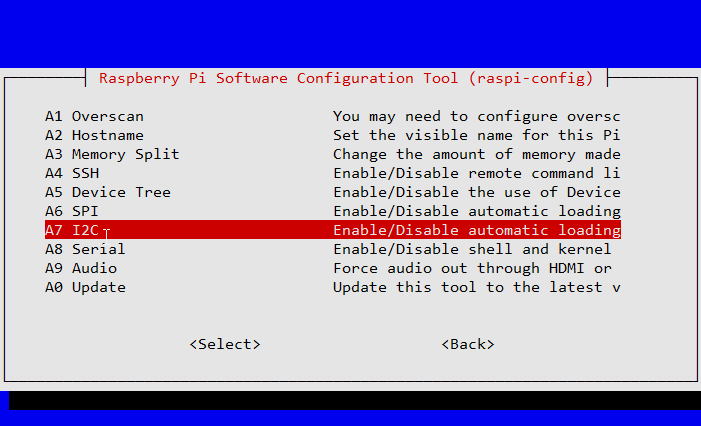
\includegraphics[width=0.7\textwidth]{raspiconfig.png}
\caption{Pantalla de configuración de las interfaces I2C y SPI.}
\label{fig:raspiconfig}
\end{center}
\end{figure}

La habilitación de estas dos interfaces, permite comunicar diferentes dispositivos que utilizan este tipo de \emph{bus de datos}. En nuestro caso, manejo de eventos táctiles, interfaz gráfica, y sensores.
De manera adicional, se procede a instalar diferentes paquetes que servirán de ayuda para realizar la plataforma de juego, como son: \texttt{i2c-tools, python-smbus, python3-smbus, python-dev, python3-dev python-gpiozero}

La documentación y los datos técnicos, así como el procedimiento de instalación, ha sido obtenido de la guía \emph{Raspberry Pi User Guide ~\cite{Upton}}.  

\subsection{Python.}
Python es un lenguaje de programación de alto nivel, multiplataforma, de tipado dinámico, multiparadigma, diseñado para ser ejecutado por intérprete. Los lenguajes de alto nivel están orientados a ofrecer al usuario, distintos algoritmos que puedan ser leídos, reorganizados e interpretados de forma sencilla, por ser más parecidos al lenguaje y a la lógica humana. Son independientes de la arquitectura del \emph{hardware}, por lo que asumen mayor portabilidad ~\cite{Python}.

La característica de tipado dinámico indica que una variable no requiere ser definida asignando su tipo de datos. Estos valores son asignados automáticamente según el valor declarado.
Se trata de un lenguaje de programación multiparadigma, al soportar orientación a objetos, programación imperativa y programación funcional ~\cite{Bahit} .

Puede ser interpretado en diversos \emph{Sistemas Operativos} como \emph{GNU/Linux, Windows, Mac OS}.
El código fuente debe ser escrito de forma estandarizada según unas reglas de estilos recogidas en \emph{Python Enhancement Proposal ~\cite{Proposal}}.

\begin{figure}[!h]
\begin{center}

\includegraphics[width=0.3\textwidth]{pythonlogo.png}
\caption{Logo de Python. Fuente: Python~\cite{Python}}
\label{fig:pythonlogo}
\end{center}
\end{figure}


\subsection{Kivy.}
\emph{Kivy} es una biblioteca de \emph{Python} de código abierto y multiplataforma, la cual ofrece un conjunto de herramientas para el desarrollo de interfaces gráficas de usuario en aplicaciones donde se requiere detectar varios eventos táctiles simultáneos.
\emph{Kivy} está escrito en \emph{Python} y \emph{Cython}, basado en \emph{OpenGL ES 2}, soporta varios dispositivos de entrada y tiene una extensa biblioteca de widgets. Con la misma base de código puede orientarse a \emph{Windows, OS X, Linux, Android e iOS}. Todos los \emph{widgets} en \emph{Kivy} están construidos con soporte multitáctil~\cite{Kivy}.

El lenguaje \textbf{Kv (Kivy)} permite crear \emph{widgets} de forma declarativa, y vincular las propiedades de los \emph{Widgets} entre sí. Ofrece una estructura del lenguaje que facilita cambios ágiles en la interfaz de usuario. Ofrece una buena separación entre la lógica de la aplicación y la interfaz de usuario.\\
\begin{figure}[!h]
\begin{center}

\includegraphics[width=0.2\textwidth]{kivylogo.png}
\caption{Logo de kivy. Fuente: Kivy ~\cite{Kivy}}
\label{fig:kivylogo}
\end{center}
\end{figure}

\subsubsection{Instalación de Kivy en Raspbian.}

Instalación de las dependencias:\\
\colorbox[gray]{0.85}{\texttt{sudo apt-get update}}\\
\colorbox[gray]{0.85}{\texttt{sudo apt-get install libsdl2-dev libsdl2-image-dev libsdl2-mixer-d libsdl2-ttf-dev \textbackslash}}\\
\colorbox[gray]{0.85}{\hspace{0.8cm} \texttt{pkg-config libgl1-mesa-dev libgles2-mesa-dev \textbackslash}}\\ 
\colorbox[gray]{0.85}{\hspace{0.8cm} \texttt{python-setuptools  libgstreamer1.0-dev git-core\textbackslash}}\\ 
\colorbox[gray]{0.85}{\hspace{0.8cm} \texttt{gstreamer1.0-plugins-\{bad,base,good,ugly\} \textbackslash}}\\
\colorbox[gray]{0.85}{\hspace{0.8cm} \texttt{gstreamer1.0-\{omx,alsa\} python-dev libmtdev-dev xclip xsel}}\\
Instalación de la última versión de \emph{Cython}:\\
\colorbox[gray]{0.85}{\texttt{sudo pip install -U Cython==0.28.2}}\\
Instalar de manera global \emph{Kivy}:\\
\colorbox[gray]{0.85}{\texttt{sudo pip install git+https://github.com/kivy/kivy.git@master
}}\\

La documentación, datos técnicos, así como el procedimiento de instalación, ha sido obtenido de la guía \emph{Kivy Documentation. User's Guide ~\cite{Kivy}}.  

\subsection{Interprete para el entorno de desarrollo Python Pycharm.}
\emph{Python} por defecto, incorpora su propio \emph{Shell} interactivo, para escribir y ejecutar código. Sin embargo, se ha optado por la instalación de un entorno de programación alternativo: \emph{PyCharm}. Este entorno ofrece ventajas sobre el \emph{Shell nativo}, como por ejemplo, poder visualizar números de línea, sangrado automático, además de ejecutar partes de código y corregir los eventuales errores.
\emph{PyCharm} es un entorno de desarrollo integrado \emph{(IDE)}\footnote{Integrated Development Environment}, multiplataforma, desarrollado por la compañía \emph{JetBrains}, para programación en lenguaje \emph{Python} ~\cite{Pycharm}.\\
\textbf{Características:}
\begin{itemize}
\item Asistencia y análisis de codificación, con finalización de código , sintaxis y resaltado de errores.
\item Navegación de proyecto y código: vistas de proyecto especializadas, vistas de estructura de archivos y saltos rápidos entre archivos, clases, métodos y usos.
\item Depurador integrado de Python.
\item Prueba de unidad integrada, con cobertura de código línea por línea.
\end{itemize}


\begin{figure}[!h]
\begin{center}

\includegraphics[width=0.2\textwidth]{pycharmlogo.png}
\caption{Logotipo PyCharm. Fuente: Pycharm ~\cite{Pycharm}}
\label{fig:pycharm}
\end{center}
\end{figure}





